\documentclass[serif]{beamer}\usepackage[]{graphicx}\usepackage[]{color}
%% maxwidth is the original width if it is less than linewidth
%% otherwise use linewidth (to make sure the graphics do not exceed the margin)
\makeatletter
\def\maxwidth{ %
  \ifdim\Gin@nat@width>\linewidth
    \linewidth
  \else
    \Gin@nat@width
  \fi
}
\makeatother

\definecolor{fgcolor}{rgb}{0.345, 0.345, 0.345}
\newcommand{\hlnum}[1]{\textcolor[rgb]{0.686,0.059,0.569}{#1}}%
\newcommand{\hlstr}[1]{\textcolor[rgb]{0.192,0.494,0.8}{#1}}%
\newcommand{\hlcom}[1]{\textcolor[rgb]{0.678,0.584,0.686}{\textit{#1}}}%
\newcommand{\hlopt}[1]{\textcolor[rgb]{0,0,0}{#1}}%
\newcommand{\hlstd}[1]{\textcolor[rgb]{0.345,0.345,0.345}{#1}}%
\newcommand{\hlkwa}[1]{\textcolor[rgb]{0.161,0.373,0.58}{\textbf{#1}}}%
\newcommand{\hlkwb}[1]{\textcolor[rgb]{0.69,0.353,0.396}{#1}}%
\newcommand{\hlkwc}[1]{\textcolor[rgb]{0.333,0.667,0.333}{#1}}%
\newcommand{\hlkwd}[1]{\textcolor[rgb]{0.737,0.353,0.396}{\textbf{#1}}}%

\usepackage{framed}
\makeatletter
\newenvironment{kframe}{%
 \def\at@end@of@kframe{}%
 \ifinner\ifhmode%
  \def\at@end@of@kframe{\end{minipage}}%
  \begin{minipage}{\columnwidth}%
 \fi\fi%
 \def\FrameCommand##1{\hskip\@totalleftmargin \hskip-\fboxsep
 \colorbox{shadecolor}{##1}\hskip-\fboxsep
     % There is no \\@totalrightmargin, so:
     \hskip-\linewidth \hskip-\@totalleftmargin \hskip\columnwidth}%
 \MakeFramed {\advance\hsize-\width
   \@totalleftmargin\z@ \linewidth\hsize
   \@setminipage}}%
 {\par\unskip\endMakeFramed%
 \at@end@of@kframe}
\makeatother

\definecolor{shadecolor}{rgb}{.97, .97, .97}
\definecolor{messagecolor}{rgb}{0, 0, 0}
\definecolor{warningcolor}{rgb}{1, 0, 1}
\definecolor{errorcolor}{rgb}{1, 0, 0}
\newenvironment{knitrout}{}{} % an empty environment to be redefined in TeX

\usepackage{alltt}
\usetheme{Boadilla}
\usepackage{graphicx}
\usepackage[final]{animate}
\usepackage{breqn}
\usepackage{xcolor}
\usepackage{booktabs}
\usepackage{tikz}
\usetikzlibrary{decorations.pathreplacing}
\usetikzlibrary{shapes,arrows,positioning,shadows}
\usepackage{subfig}
\usepackage{pgf}

% change format of enumerated lists
\setbeamertemplate{enumerate items}[default]

\setbeamertemplate{navigation symbols}{}

%tikz objects
\tikzstyle{decision} = [diamond, draw, text width=6em, text badly centered, inner sep=2pt, top color=white, bottom color=zissou3]
\tikzstyle{block} = [rectangle, draw, text width=10em, text centered, rounded corners, minimum height=3em, minimum width=8em, top color = white, bottom color=zissou3]
\tikzstyle{declare} = [rectangle, draw, text width=10em, text centered, minimum height=3em, minimum width=8em, top color = white, bottom color=zissou3]

% knitr setup


% dependent data


% custom colors
\definecolor{zissou1}{HTML}{3B9AB2}\definecolor{zissou2}{HTML}{78B7C5}\definecolor{zissou3}{HTML}{EBCC2A}\definecolor{zissou4}{HTML}{E1AF00}\definecolor{zissou5}{HTML}{F21A00}

% my custom ggplot theme


% figure used on title page


\setbeamercolor{title}{fg=zissou1} % main title
\setbeamercolor{frametitle}{fg=zissou3, bg=zissou2} % frame titles
\setbeamercolor{structure}{fg=zissou5} % bottom banner
\setbeamercolor{normal text}{fg=zissou1}
\usebackgroundtemplate{
\includegraphics[height=\paperheight,width=\paperwidth]{fig/back_tmp.pdf}}
\IfFileExists{upquote.sty}{\usepackage{upquote}}{}
\begin{document}

\title[WRTDS in Tidal Waters]{\textbf{Adaptation of WRTDS to characterize chlorophyll trends in tidal waters}}
\author[M. Beck]{Marcus W. Beck\inst{1} \and James D. Hagy III\inst{2}}

\institute[ORISE, EPA]{\inst{1} ORISE post-doc, USEPA National Health and Environmental Effects Research Laboratory, Gulf Ecology Division, \href{mailto:beck.marcus@epa.gov}{beck.marcus@epa.gov} \and \inst{2} USEPA National Health and Environmental Effects Research Laboratory, Gulf Ecology Division, \href{mailto:hagy.jim@epa.gov}{hagy.jim@epa.gov}}

\date{}

\titlegraphic{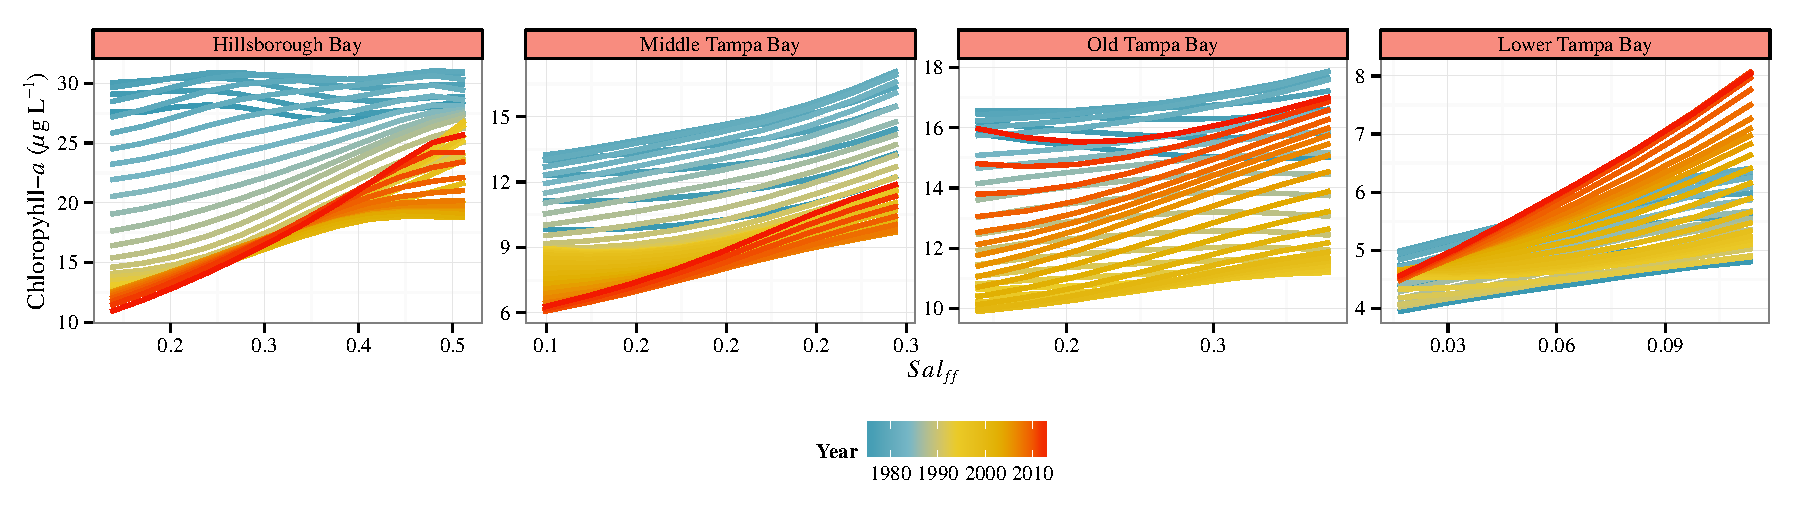
\includegraphics[width=0.85\linewidth]{fig/title_plo.pdf}}

%%%%%%
\begin{frame}[shrink]
\titlepage
\end{frame}

%%%%%%
\begin{frame}{\textbf{The eutrophication paradigm}}{\textbf{Research and management in coastal waters}}
\begin{quote}
Eutrophication (noun) - an \alert{increase} in the rate of supply of \alert{organic matter} to an ecosystem\\~\\
\vspace{0.05in}
\hfill -- \cite{Nixon95}
\end{quote}
\begin{center}
\scalebox{1}{
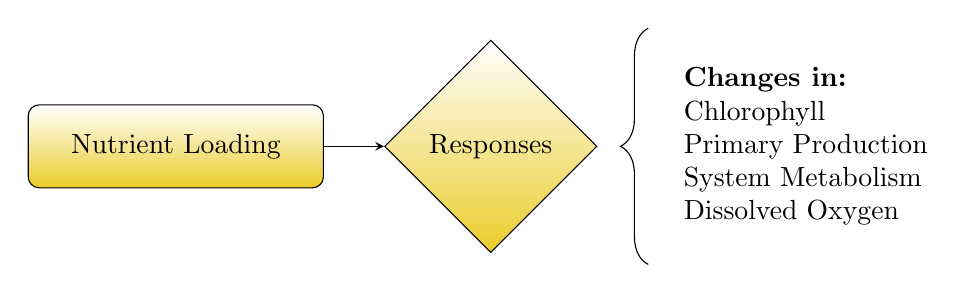
\begin{tikzpicture}[node distance = 4cm, auto, >=stealth]
  \node[block] (a) {Nutrient Loading};
	\node[decision] (b)  [right of=a] {Responses};
 	\draw[->] (a) -- (b);
  \draw[decorate,decoration={brace,amplitude=10pt}] [right of=b] (2,-1.5) -- (2,1.5);
  \node[draw,align=left,draw=none] [right of=b] {\textbf{Changes in:}\\ Chlorophyll\\ Primary Production\\ System Metabolism\\ Dissolved Oxygen};
\end{tikzpicture}}
\end{center}
\vspace{-0.5cm}\hspace*{15pt}\scalebox{0.7}{\hbox{\tiny Adapted from \cite{Cloern01}}}\\~\\
\end{frame}

%%%%%%
\begin{frame}{\textbf{The eutrophication paradigm}}{\textbf{Research and management in coastal waters}}
Human inputs can greatly accelarate eutrophication... particularly for coastal waters \\~\\
\begin{itemize}
\item Depletion of bottom water dissolved oxygen \cite{Diaz08}
\item Increase in frequency/severity of harmful algal blooms \cite{Glibert13}
\item Reduction or extirpation of seagrass communities \cite{Tomasko05}
\item Propogated effects to upper trophic levels \cite{Powers05}
\end{itemize}
\end{frame}

%%%%%%
\begin{frame}{\textbf{The eutrophication paradigm}}{\textbf{Challenges for criteria development}}
There are challenges to providing guidance...\\~\\
\alert{Challenge 1:} We don't fully understand eutrophication processes \\~\\
\begin{quote}
There are good reasons to believe that eutrophication will, in the near \alert{future}, become a \alert{hazard in marine coastal areas} in many parts of the world.\\~\\
\vspace{0.05in}
\hfill -- \cite{Rosenberg85} \\~\\
\end{quote}
\end{frame}

%%%%%
\begin{frame}{\textbf{The eutrophication paradigm}}{\textbf{Challenges for criteria development}}
Our conceptual model for understanding the effects of nutrient pollution is adopted from freshwater sciences. \\~\\
\begin{center}
\scalebox{1}{
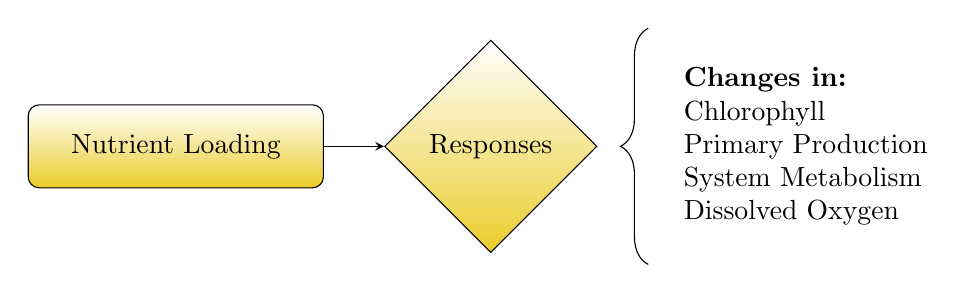
\begin{tikzpicture}[node distance = 4cm, auto, >=stealth]
  \node[block] (a) {Nutrient Loading};
	\node[decision] (b)  [right of=a] {Responses};
 	\draw[->] (a) -- (b);
  \draw[decorate,decoration={brace,amplitude=10pt}] [right of=b] (2,-1.5) -- (2,1.5);
  \node[draw,align=left,draw=none] [right of=b] {\textbf{Changes in:}\\ Chlorophyll\\ Primary Production\\ System Metabolism\\ Dissolved Oxygen};
\end{tikzpicture}}
\end{center}
\vspace{-0.5cm}\hspace*{15pt}\scalebox{0.7}{\hbox{\tiny Adapted from \cite{Cloern01}}}\\~\\
\end{frame}



\begin{frame}{\textbf{The eutrophication paradigm}}{\textbf{Challenges for criteria development}}
Spatial and temporal variation in chlorophyll for Tampa Bay\\~\\
\begin{columns}
\begin{column}{0.53\textwidth}
\begin{center}
\includegraphics<1>[width=\textwidth,trim=0in 0.2in 0.6in 0in]{fig/ggchl_1.pdf}
\includegraphics<2>[width=\textwidth,trim=0in 0.2in 0.6in 0in]{fig/ggchl_2.pdf}
\includegraphics<3>[width=\textwidth,trim=0in 0.2in 0.6in 0in]{fig/ggchl_3.pdf}
\includegraphics<4>[width=\textwidth,trim=0in 0.2in 0.6in 0in]{fig/ggchl_4.pdf}
\includegraphics<5>[width=\textwidth,trim=0in 0.2in 0.6in 0in]{fig/ggchl_5.pdf}
\end{center}
\end{column}
\begin{column}{0.43\textwidth}
\begin{center}
\includegraphics<1>[width=\textwidth]{fig/wbid_map_1.pdf}
\includegraphics<2>[width=\textwidth]{fig/wbid_map_2.pdf}
\includegraphics<3>[width=\textwidth]{fig/wbid_map_3.pdf}
\includegraphics<4>[width=\textwidth]{fig/wbid_map_4.pdf}
\includegraphics<5>[width=\textwidth]{fig/wbid_map_5.pdf}
\end{center}
\end{column}
\end{columns}
\end{frame}

%%%%%%
\begin{frame}{\textbf{The eutrophication paradigm}}{\textbf{Challenges for criteria development}}
\alert{Challenge 2:} We have the data but often lack tools to unambiguously and quantitatively characterize\\~\\
\vspace{0.2in}
\begin{quote}
Data without models are chaos, but models without data are fantasy. \\~\\
\vspace{0.05in}
\hspace{0.1in}-- NWQMC 2014 plenary, R. Hirsch via \cite{Nisbet14}
\end{quote}
\end{frame}

%%%%%%
\begin{frame}{\textbf{Tampa Bay}}{\textbf{Understanding chlorophyll response to eutrophication}}
\begin{block}{Study objective}
Adapt and apply nutrient response model for estuaries that leverages the descriptive capabilities of large datasets \scriptsize [Beck and Hagy, in review]
\end{block}
\vspace{0.2in}
Questions of management concern -- Can we...
\begin{itemize}
\item ...provide a natural history of water quality that is temporally consistent with drivers of change?
\item ...characterize changes in extreme events in addition to describing the mean response?  
\item ...improve our understanding of the nutrient-response paradigm in estuaries?
\end{itemize}
\end{frame}

% tampa bay map, w/ inset


%%%%%%
\begin{frame}{\textbf{Tampa Bay}}{\textbf{Understanding chlorophyll response to eutrophication}}
\begin{columns}
\begin{column}{0.5\textwidth}
\begin{itemize}
\item Four bay segments\\~\\
\item Monthly wq data at 50 stations from 1974 to present \\~\\
\item Longitudinal profile of nutrient load and salinity \\~\\
\end{itemize}
\vspace{0cm}\hspace*{15pt}\scalebox{0.7}{\hbox{\tiny Data from \cite{TBEP11}}}
\end{column}
\begin{column}{0.5\textwidth}
\centerline{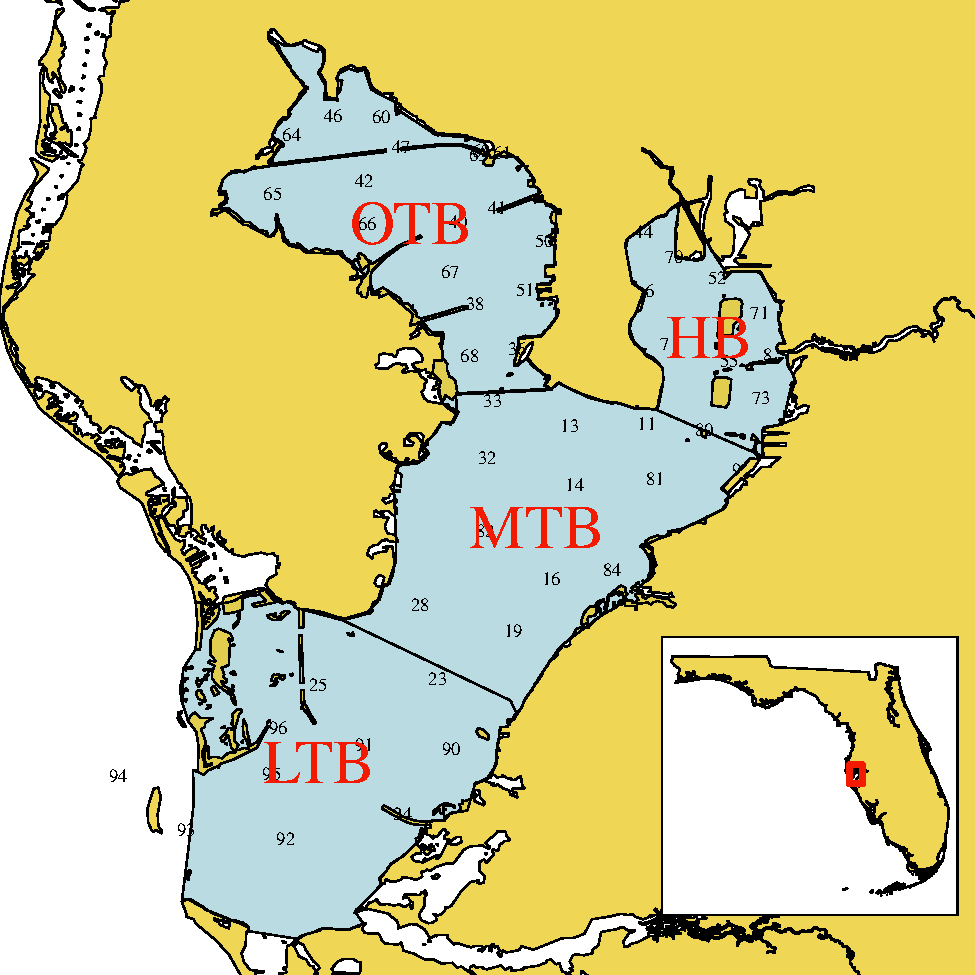
\includegraphics[width = \textwidth]{fig/tb_map.pdf}}
\end{column}
\end{columns}
\end{frame}

%%%%%%
\begin{frame}{\textbf{Tampa Bay}}{\textbf{Understanding chlorophyll response to eutrophication}}
\begin{figure}[!ht]


{\centering 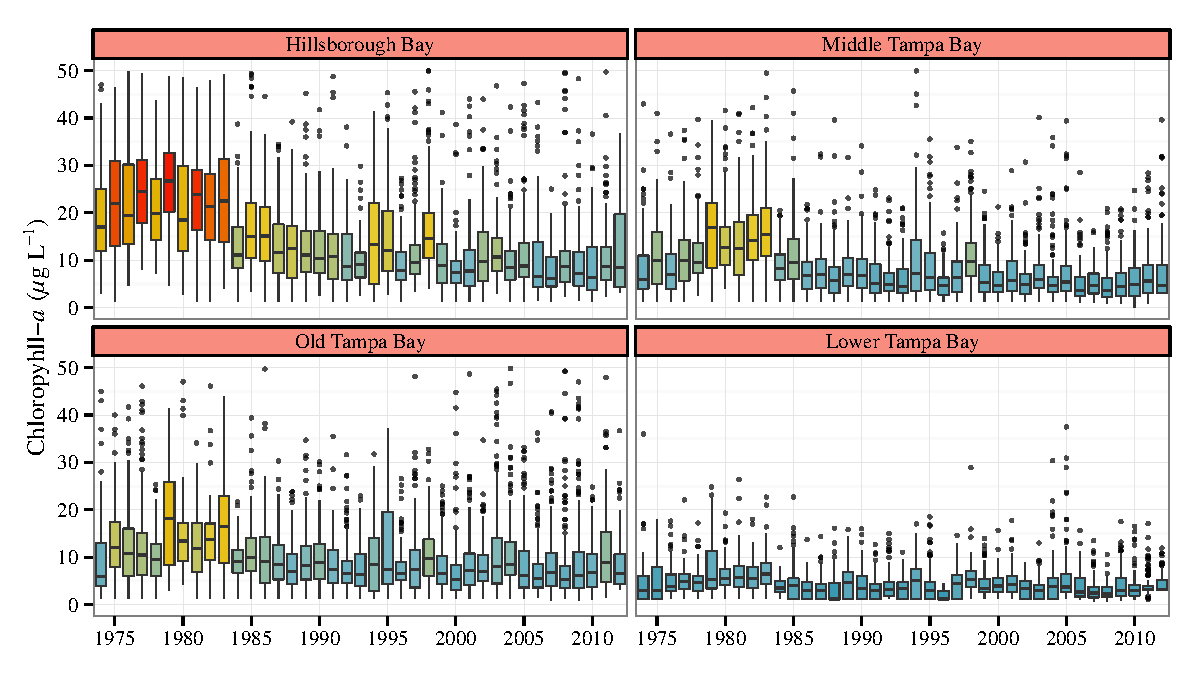
\includegraphics[width=\linewidth]{fig/annual_chl} 

}

\caption[Annual trends in chlorophyll for each bay segment]{Annual trends in chlorophyll for each bay segment.\label{fig:annual_chl}}
\end{figure}


\end{frame}

% variation in chl by year, season, and management

%%%%%%
\begin{frame}{\textbf{Tampa Bay}}{\textbf{Understanding chlorophyll response to eutrophication}}
What affects our interpretation of chlorophyll response to nutrients?
\vspace{-0.1in}
\captionsetup[subfloat]{captionskip=0pt, position=top}
\begin{figure}
\centering
\subfloat[]{
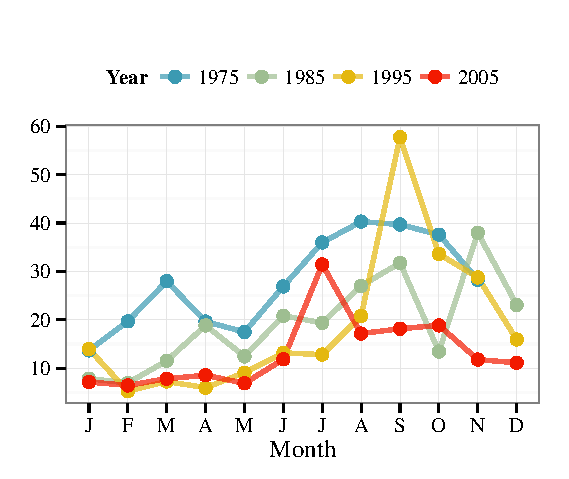
\includegraphics[width=0.46\textwidth,page=1,trim=0.2in 0in 0in 0.35in,clip]{fig/salmoyr.pdf}
\label{fig:salmoyr1}
}
\subfloat[]{
\includegraphics[width=0.46\textwidth,page=2,trim=0.2in 0in 0in 0.35in,clip]{fig/salmoyr.pdf}
\label{fig:salmoyr2}
}

\leavevmode\smash{\makebox[0pt]{\hspace{0em}% HORIZONTAL POSITION           
  \rotatebox[origin=l]{90}{\hspace{3em}% VERTICAL POSITION
    {\color{black} Chlorophyll-\textit{a}}}}}
    \hspace{0pt plus 1filll}\null

\caption{Variation in chlorophyll by {\color{zissou5}\protect\subref{fig:salmoyr1}} time and {\color{zissou5}\protect\subref{fig:salmoyr2}} salinity and management in Hillsborough Bay.  Panel {\color{zissou5}\protect\subref{fig:salmoyr1}} is colored before and after wastewater treatment in 1979.}
\label{fig:salmoyr}
\end{figure}
\captionsetup[subfloat]{position=top}
\end{frame}

%%%%%%
\begin{frame}{\textbf{Tampa Bay}}{\textbf{Understanding chlorophyll response to eutrophication}}
The \alert{weighted regression (WRTDS)} model is being developed by USGS for pollutant modelling in rivers \cite{Hirsch10}\\~\\
Based on the idea that pollution concentration is a function of \alert{time}, \alert{discharge}, and \alert{season}\\~\\
\alert{Problem:} We want to see if management has an effect on reducing pollutant load over time, but pollutant load varies with discharge.\\~\\
\alert{Solution:} Develop a model that accounts for changes in relationships between drivers of pollution over time.\\~\\
\alert{Adaptation:} Can this approach be used to evaluate chlorophyll trends in Tampa Bay?
\end{frame}

%%%%%%
\begin{frame}{\textbf{Weighted regression approach}}{\textbf{ Adaptation to estuaries}}
The \alert{weighted regression (WRTDS)} model is being developed by USGS for pollutant modelling in fluvial systems \cite{Hirsch10}\\~\\
Based on the idea that pollution concentration is a function of \alert{time}, \alert{discharge}, and \alert{season}\\~\\
\begin{block}{WRTDS functional form}
\centerline{\textbf{$
\ln\left(c\right) = \beta_0 + \beta_1 t + \beta_2 \ln\left(Q\right) + \beta_3 \sin\left(2\pi t\right) + \beta_4 \cos\left(2\pi t\right) + \epsilon $
}}
\end{block}
\vspace{0.1in}
Logical extension to estuary eutrophication\\~\\
\begin{block}{Adapted functional form}
\centerline{\textbf{$
\ln\left(Chl\right) = \beta_0 + \beta_1 t + \beta_2 Sal_{ff} + \beta_3 \sin\left(2\pi t\right) + \beta_4 \cos\left(2\pi t\right) + \epsilon $
}}
\end{block}
\end{frame}



%%%%%%
\begin{frame}{\textbf{Tampa Bay}}{\textbf{Understanding chlorophyll response to eutrophication}}
How does weighted regression work?
\begin{center}
\animategraphics[controls,width=\linewidth]{12}{fig/wtex}{}{} %frame rate is 12 per/sec
\end{center}
\end{frame}

%%%%%%
\begin{frame}{\textbf{Tampa Bay}}{\textbf{Understanding chlorophyll response to eutrophication}}
This gives us improved predictions of chlorophyll dynamics...
\begin{figure}[!ht]


{\centering 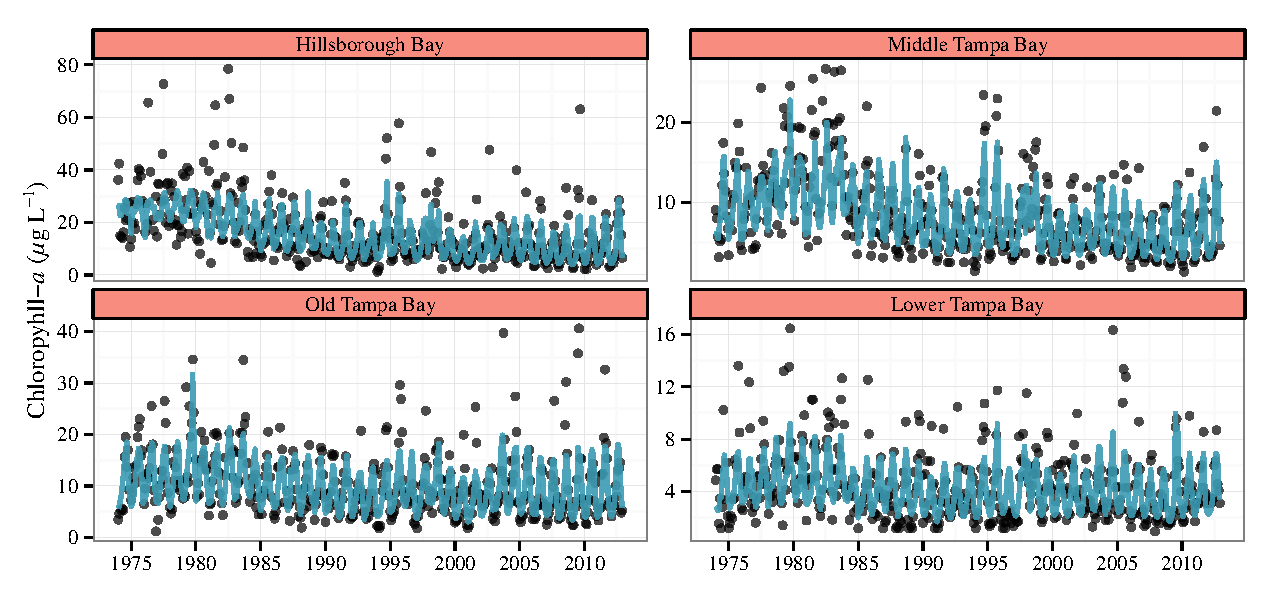
\includegraphics[width=\linewidth]{fig//predvals} 

}

\caption[Predicted and observed monthly chlorophyll by segment]{Predicted and observed monthly chlorophyll by segment.\label{fig:/predvals}}
\end{figure}


\end{frame}

%%%%%%
\begin{frame}{\textbf{Weighted regression approach}}{\textbf{ Results for Tampa Bay}}
\vspace{-0.07in}
%latex.default(null.dat, file = "", caption.loc = "top", caption = cap.val,     cgroup = c("mean", "0.9 $\\tau$", "0.1 $\\tau$"), n.cgroup = c(2,         2, 2), colheads = rep(c("Non-wtd", "Wtd"), 3), rowlabel = "Statistic",     rowname = stat, n.rgroup = rep(2, 4), rgroup = segs, label = "tab:modperf",     digits = 2, size = "footnotesize", col.just = rep("l", ncol(null.dat)))%
\begin{table}[!tbp]
{\footnotesize
\caption{Fit statistics by bay segment comparing non-weighted and weighted regression.\label{tab:modperf}} 
\begin{center}
\begin{tabular}{lllcllcll}
\hline\hline
\multicolumn{1}{l}{\bfseries Statistic}&\multicolumn{2}{c}{\bfseries mean}&\multicolumn{1}{c}{\bfseries }&\multicolumn{2}{c}{\bfseries 0.9 $\tau$}&\multicolumn{1}{c}{\bfseries }&\multicolumn{2}{c}{\bfseries 0.1 $\tau$}\tabularnewline
\cline{2-3} \cline{5-6} \cline{8-9}
\multicolumn{1}{l}{}&\multicolumn{1}{c}{Non-wtd}&\multicolumn{1}{c}{Wtd}&\multicolumn{1}{c}{}&\multicolumn{1}{c}{Non-wtd}&\multicolumn{1}{c}{Wtd}&\multicolumn{1}{c}{}&\multicolumn{1}{c}{Non-wtd}&\multicolumn{1}{c}{Wtd}\tabularnewline
\hline
{\bfseries HB}&&&&&&&&\tabularnewline
~~$R^2$&$0.54$&$0.66$&&$0.32$&$0.47$&&$0.31$&$0.45$\tabularnewline
~~$RMSE$&$0.48$&$0.41$&&$0.78$&$0.66$&&$0.74$&$0.67$\tabularnewline
\hline
{\bfseries OTB}&&&&&&&&\tabularnewline
~~$R^2$&$0.54$&$0.65$&&$0.29$&$0.45$&&$0.34$&$0.47$\tabularnewline
~~$RMSE$&$0.41$&$0.36$&&$0.65$&$0.61$&&$0.67$&$0.59$\tabularnewline
\hline
{\bfseries MTB}&&&&&&&&\tabularnewline
~~$R^2$&$0.60$&$0.71$&&$0.34$&$0.51$&&$0.38$&$0.51$\tabularnewline
~~$RMSE$&$0.37$&$0.31$&&$0.60$&$0.52$&&$0.61$&$0.52$\tabularnewline
\hline
{\bfseries LTB}&&&&&&&&\tabularnewline
~~$R^2$&$0.40$&$0.51$&&$0.26$&$0.37$&&$0.18$&$0.34$\tabularnewline
~~$RMSE$&$0.45$&$0.40$&&$0.72$&$0.65$&&$0.77$&$0.68$\tabularnewline
\hline
\end{tabular}\end{center}}

\end{table}

\end{frame}

%%%%%%
\begin{frame}{\textbf{Weighted regression approach}}{\textbf{ Results for Tampa Bay}}
Results can also be normalized by predictors -- salinity
\begin{figure}[!ht]


{\centering 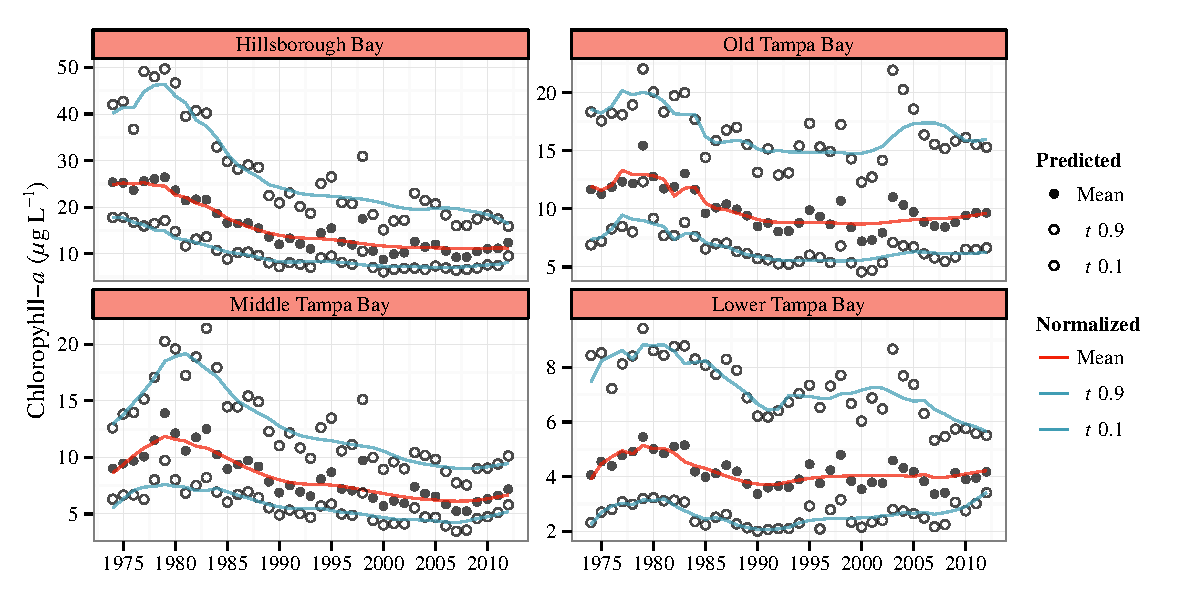
\includegraphics[width=\linewidth]{fig//prednrm} 

}

\caption[Predicted and salinity-normalized annual chlorophyll by segment]{Predicted and salinity-normalized annual chlorophyll by segment.\label{fig:/prednrm}}
\end{figure}


\end{frame}



%%%%%%
\begin{frame}{\textbf{Tampa Bay}}{\textbf{Understanding chlorophyll response to eutrophication}}
Because the model is dynamic, we have parameters describing the relationship of chlorophyll with other factors specific to different time periods \\~\\
\begin{columns}[T]
\begin{column}{0.45\textwidth}
\centerline{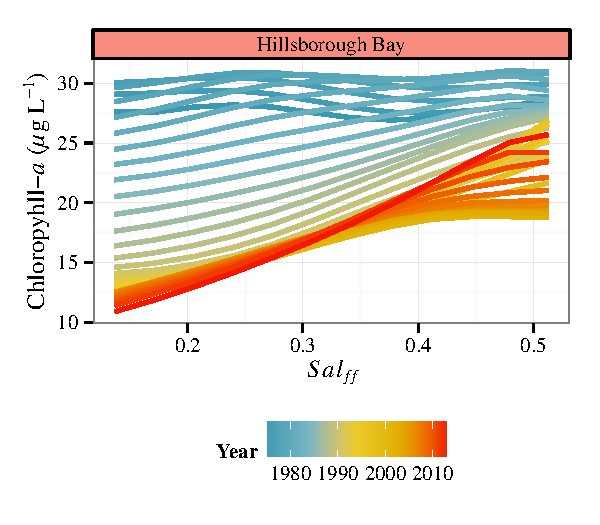
\includegraphics[width = \textwidth]{fig/hill.pdf}}
\end{column}
\begin{column}{0.45\textwidth}
\begin{itemize}
\item Early period (blue) - point-sources
\item Late period (red) - non-point sources
\item Chlorophyll shows increasing response to freshwater input in recent years
\end{itemize}
\end{column}
\end{columns}
\end{frame}

%%%%%%
\begin{frame}{\textbf{Tampa Bay}}{\textbf{Understanding chlorophyll response to eutrophication}}
What does this mean for Tampa Bay and elsewhere?\\~\\
\begin{itemize}
\item Predictions followed observed chlorophyll -- but increased clarity in the description
\item More detailed evaluation of trends allows greater insight into drivers of change\\~\\
\end{itemize}
The model parameters show us a picture...
\centerline{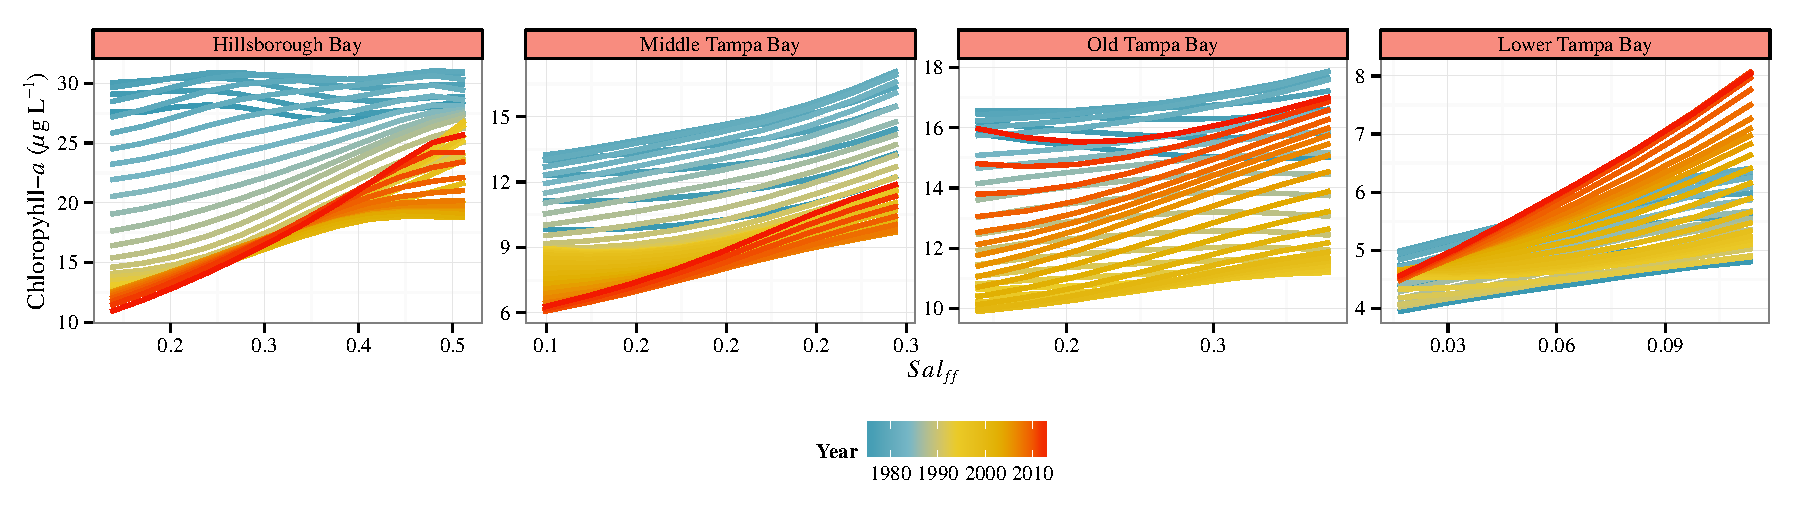
\includegraphics[width = \textwidth]{fig/title_plo.pdf}}
\end{frame}

%%%%%%
\begin{frame}{\textbf{Weighted regression approach}}{\textbf{ General conclusions}}
Adaptation of freshwater modelling approaches to estuaries suggests improved interpretation of trends is possible\\~\\
A data-driven process for investigational analysis - can't ask `why' without the `what'\\~\\
Results can improve our understanding of the coastal model of eutrophication
\begin{center}
\scalebox{1}{
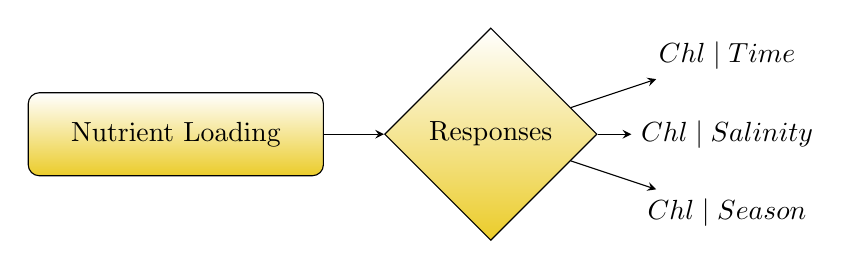
\begin{tikzpicture}[node distance = 7em, auto, >=stealth]
  \node[block] (a) {Nutrient Loading};
  \node[decision] (b)  [right of=a, node distance = 4cm] {Responses};
   \draw[->] (a) -- (b);	
  \node[draw,draw=none] (c) at(7,1) {\alert{$Chl \mid Time$}};
  \node[draw,draw=none] (d) at(7,0) {\alert{$Chl \mid Salinity$}};
  \node[draw,draw=none] (e) at(7,-1) {\alert{$Chl \mid Season$}};
  \draw[->] (b) -- (c);
  \draw[->] (b) -- (d);
  \draw[->] (b) -- (e);
\end{tikzpicture}}
\end{center}
\end{frame}

%%%%%%
\begin{frame}
Acknowledgments:\\~\\
\begin{columns}
\begin{column}{0.6\textwidth}
{\footnotesize
Research staff and employees at USEPA Gulf Ecology Division - especially J. Hagy, M. Murrell\\~\\
Field staff and data managers at Hillsborough County Environmental Protection Commission\\~\\
Research coordinators, technicians, and field staff of the National Estuarine Research Reserve System}\\~\\
\end{column}
\begin{column}{0.3\textwidth}
\vspace{-0.2in}
\begin{center}
{\tiny
Wes Anderson Zissou color theme borrowed and adapted from \href{https://github.com/karthik/wesanderson}{github.com/karthik}\\~\\
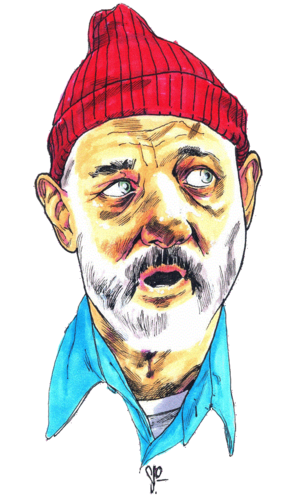
\includegraphics[width=0.55\linewidth]{fig/zissou.png}\\~\\
\vspace{-0.15in}
\scalebox{0.7}{\hbox{\tiny Image credit:\thinspace{\tiny \href{http://stephenmorrow.deviantart.com/}{Stephen Morrow}}}}}
\end{center}
\end{column}
\end{columns}
\vfill
Funding sources and contact:\\~\\
\begin{columns}
\begin{column}{0.5\textwidth}
\centerline{
\includegraphics[width=0.4\linewidth]{fig/epa_logo.png}}
\end{column}
\begin{column}{0.5\textwidth}
\scriptsize
\href{mailto:beck.marcus@epa.gov}{beck.marcus@epa.gov} \\~\\
Phone: 8509342480 \\~\\
Github: \href{https://github.com/fawda123/}{github.com/fawda123/} \\~\\
Blog: \href{http://beckmw.wordpress.com/}{beckmw.wordpress.com/}
\end{column}
\end{columns}
\vspace{0.2in}
\end{frame}

%%%%%%
\begin{frame}[allowframebreaks,t]{\textbf{References}}
\tiny
\setbeamertemplate{bibliography item}{}
\bibliographystyle{apalike_mine}
\bibliography{ref_diss}
\end{frame}

\end{document}
